\documentclass[12pt]{article}
 
\usepackage[margin=1in]{geometry} 
\usepackage{amsmath,amsthm,amssymb}
\usepackage{hyperref}
\usepackage{graphicx}
\usepackage{xcolor}
\usepackage[many]{tcolorbox}
\tcbuselibrary{listings}
\usepackage{listings}

\definecolor{lg}{HTML}{f0f0f0}

\newtcblisting{pycode}{
    colback=lg,
    boxrule=0pt,
    arc=0pt,
    outer arc=0pt,
    top=0pt,
    bottom=0pt,
    colframe=white,
    listing only,
    left=15.5pt,
    enhanced,
    listing options={
        basicstyle=\small\ttfamily,
        keywordstyle=\color{blue},
        language=Python,
        showstringspaces=false,
        tabsize=2,
        numbers=left,
        breaklines=true
    },
    overlay={
        \fill[gray!30]
        ([xshift=-3pt]frame.south west)
        rectangle
        ([xshift=11.5pt]frame.north west);
    }
}

\lstset{
    language=Python,
    basicstyle=\small\ttfamily,
}

 
\begin{document}
 
\title{Exercise 3}
\author{Cristian Manuel Abrante Dorta - 888248\\
ELEC-E8125 - Reinforcement Learning}

\maketitle
\section{Cartpole}

\subsection{Task 1: Implement Q-learning for the Cartpole environment. Compare using a constant value of $\epsilon$ = 0.2 to reduce the value of $\epsilon$ over time}

The comparison of the results between the two versions of the Q-learning algorithm (for different values of $\epsilon$) was done by observing the plot of the average timesteps that the execution achieved, and also by observing the execution of the cart pole with the trained model.

\subsubsection{$\epsilon$ fixed to 0.2}

Running the Q learning algorithm for the fixed value of $\epsilon=0.2$ for 20000 episodes, gave, as a result, the following plot of the average timesteps length:

\begin{figure}[h]
    \centering
    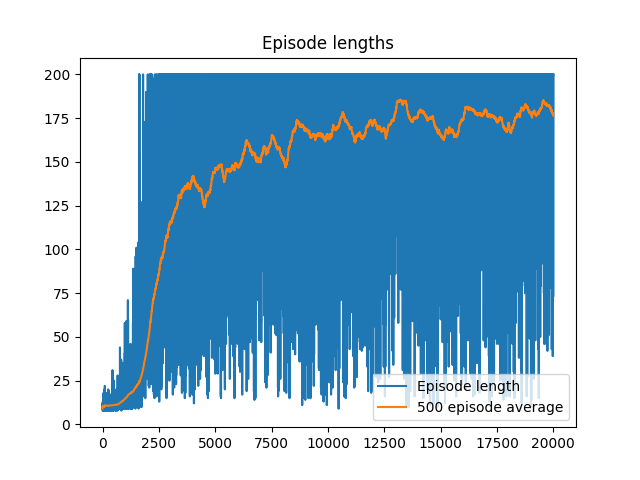
\includegraphics[scale=0.6]{exercise-3/plots/episodes-fixed-0.2.png}
    \caption{Average timesteps for the Q-Learning algorithm}
    \label{fig:fixed-0.2}
\end{figure}

In figure \ref{fig:fixed-0.2} is shown the evolution of the timesteps that the model is able to achieve over the training episodes. Variance is really significant over the executions, but the average tendency is to increase, reaching almost a stabilization level from episode 15000.\\

\subsubsection{GLIE $\epsilon$}

For the \textit{greedy in limit with infinite exploration} technique, the $\epsilon$ variable was set according to this formula:

\begin{equation}
    \epsilon = \frac{a}{a + p}
\end{equation}

Where each variable meant:

\begin{itemize}
    \item $p$: Current episode of the training execution.
    \item $a$: This is the constant integer variable used for the decrement of the epsilon over the training episodes. The value was established in a way that in the final execution, the $\epsilon$ variable will be 0.1:
    \begin{equation}
        a = \frac{\epsilon}{1 - \epsilon}p; \quad \quad a = \frac{0.1}{1-0.1}\cdot20000; \quad \quad a = 2222
    \end{equation}
\end{itemize}

Having this formula specified, we can execute the training, observing the corresponding plot for the average timesteps:

\begin{figure}[h]
    \centering
    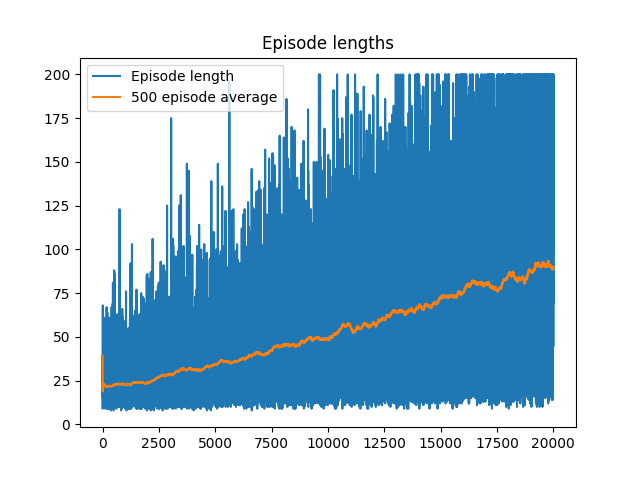
\includegraphics[scale=0.6]{exercise-3/plots/episodes-variable-0.0.png}
    \caption{Average timesteps for the Q-Learning algorithm}
    \label{fig:variable}
\end{figure}

As we can see in figure \ref{fig:variable}, the tendency of the average timesteps is to increase over the episodes, performing slightly better compared to the fixed value of $\epsilon$ (Figure \ref{fig:fixed-0.2}). \\

As there is only a small difference between the performance of both algorithms (even though the GLIE is better), both of the executions in the cart pole environment lead to successful results, having an agent that is capable of balancing the pole all over the timesteps.

\subsection{Task 2: Plot the optimal value function of each state}

After the execution of the training for both types of algorithms, we can plot the optimal value for each state:

\begin{figure}[ht]
    \centering
   \begin{minipage}{0.48\textwidth}
     \centering
     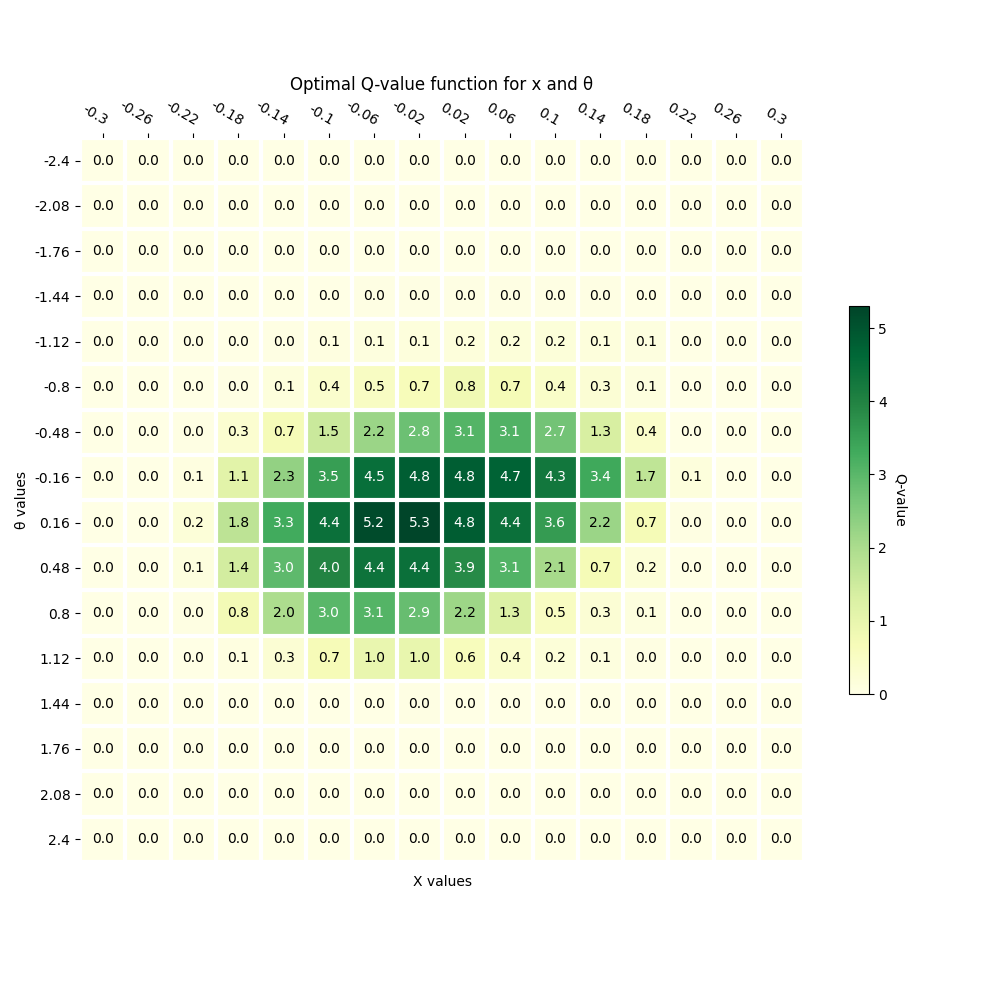
\includegraphics[width=0.9\linewidth]{exercise-3/plots/heatmap-fixed-0.2.png}
     \caption{Heatmap of the optimal Q-value for $\epsilon=0.2$}
     \label{fig:task-2-1}
   \end{minipage}\hfill
   \begin{minipage}{0.48\textwidth}
     \centering
     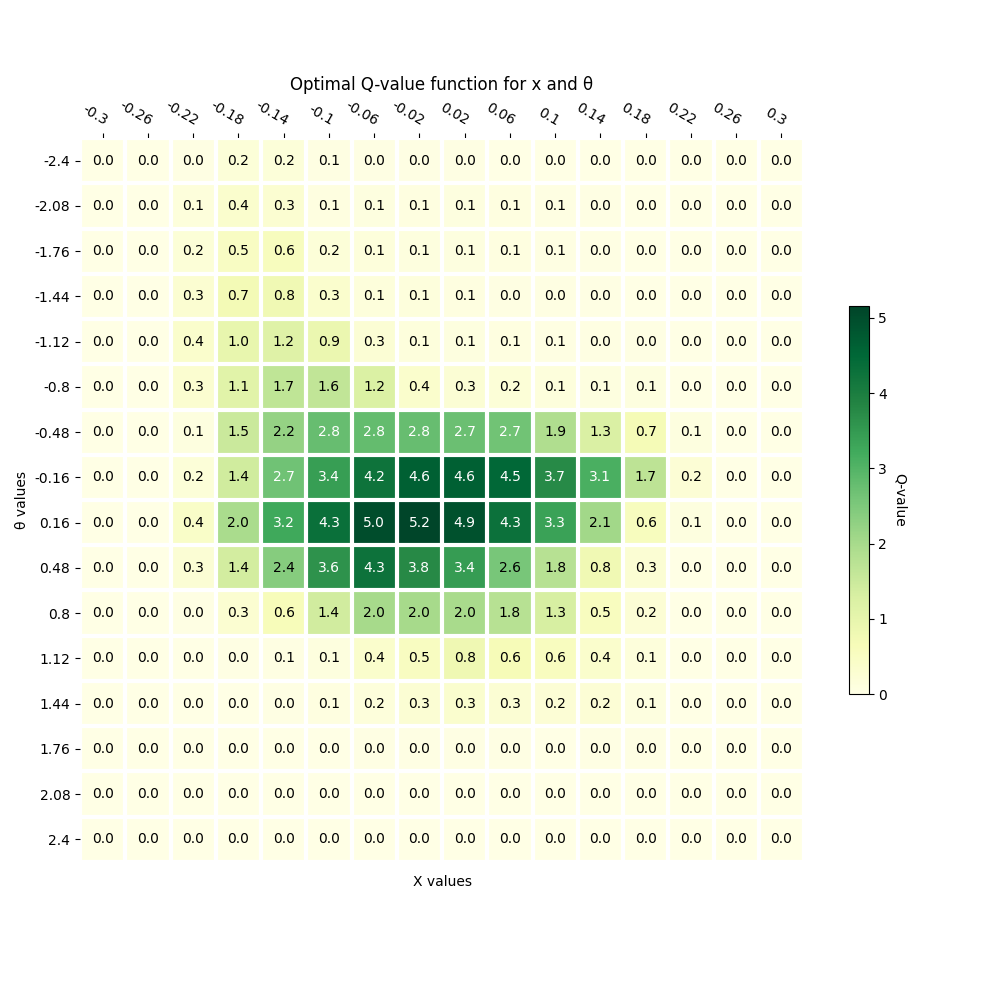
\includegraphics[width=0.9\linewidth]{exercise-3/plots/heatmap-variable-0.0.png}
     \caption{Heatmap of the optimal Q-value for variable $\epsilon$}
     \label{fig:task-2-2}
   \end{minipage}
\end{figure}

In those plots the difference between both algorithms is well seen. In the $\epsilon$-fixed version (Figure \ref{fig:task-2-1}), we can see that the exploration of the state space is limited because the agent is greedy more frequently.\\

On the variable $\epsilon$ version (Figure \ref{fig:task-2-2}), we can notice that even though there is a concentration in the selected actions, the state space has more states explored. This is because in the initial phases of the training the $\epsilon$ value has a high value, so random actions are selected in many situations.

\subsection{Question 1: What do you think the heatmap would have looked like}

\subsubsection{before the training?}

Before the training, the heatmap can only contain the initial value of the q-grid, which for the case of tasks 1 and 2 is going to be value 0. So the heatmap will be a 16x16 grid with all the values filled to 0. \\

This could be confirmed practically, executing the algorithm with a fixed $\epsilon = 0.2$, and printing the grid before the first episode (Figure \ref{fig:q-1-1}).

\begin{figure}[h]
    \centering
    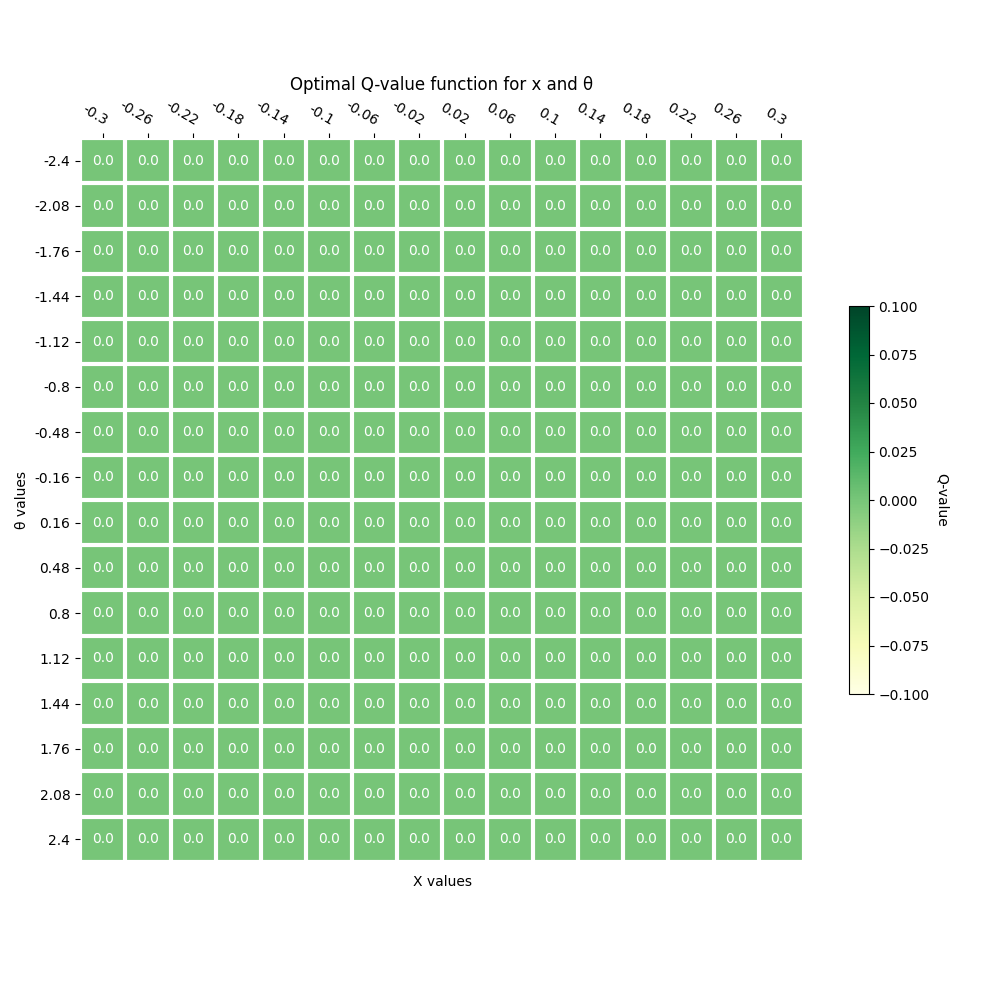
\includegraphics[scale=0.25]{exercise-3/plots/heatmap-fixed-0.2-ep-0.png}
    \caption{Q-grid in episode 0}
    \label{fig:q-1-1}
\end{figure}

\subsubsection{after a single episode?}

After the first episode, the heatmap will only include the explored positions in the first executions, which will be probably the ones near the central position of the agent at the beginning (near the value 0.0 for $x$).\\

As in the previous section, we have included the practical execution for fixed $\epsilon=0.2$

\begin{figure}[h]
    \centering
    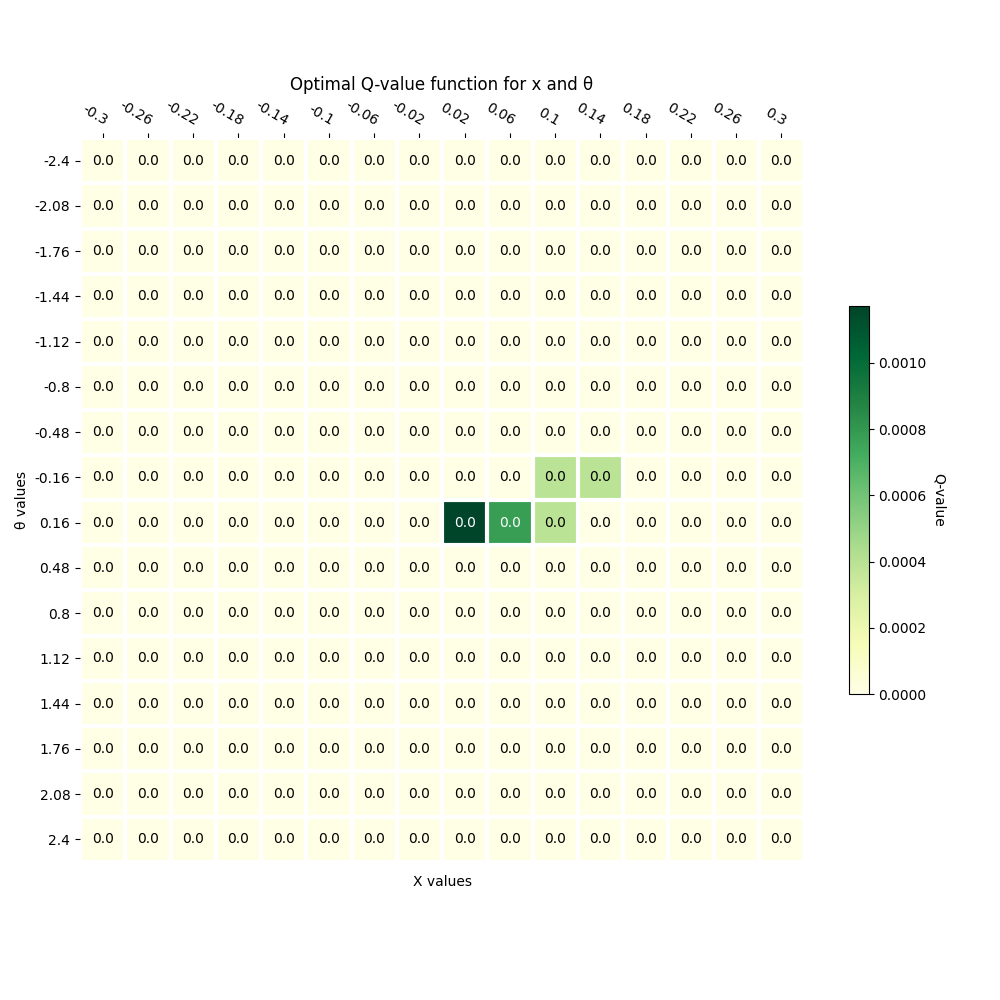
\includegraphics[scale=0.25]{exercise-3/plots/heatmap-fixed-0.2-ep-1.png}
    \caption{Q-grid in episode 1}
    \label{fig:q-1-2}
\end{figure}

\subsubsection{halfway through the training?}

In the halfway of the training, the states with higher q-value should be in the center of the grid, because they have been explored probably more times. At the same time, compared with the execution in one episode, there should be more states with set q-values.\\

Figure \ref{fig:q-1-3} is the practical example of it:

\begin{figure}[h]
    \centering
    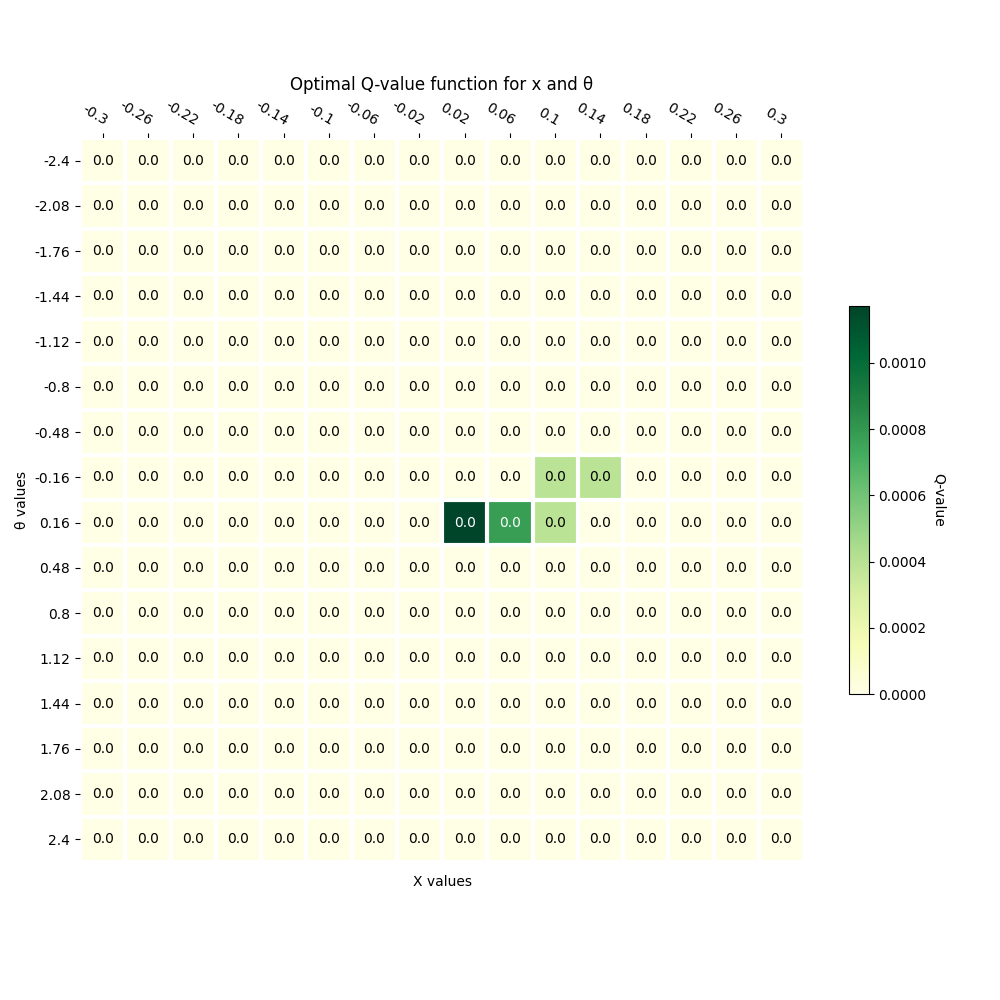
\includegraphics[scale=0.25]{exercise-3/plots/heatmap-fixed-0.2-ep-1.png}
    \caption{Q-grid in episode 10000}
    \label{fig:q-1-3}
\end{figure}

\subsection{Task 3: Set $\epsilon$ to zero, effectively making the policy greedy w.r.t. current Q-value estimates.}

If the policy is set as effectively greedy (setting $\epsilon = 0$), then those plots are obtained for the average timesteps in the training process:

\begin{figure}[ht]
    \centering
   \begin{minipage}{0.48\textwidth}
     \centering
     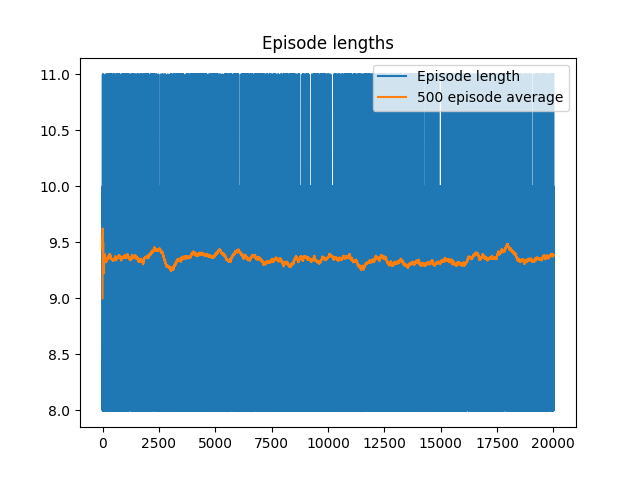
\includegraphics[width=0.9\linewidth]{exercise-3/plots/episodes-fixed-0.0.png}
     \caption{Heatmap of the optimal Q-value for $\epsilon=0.2$}
     \label{fig:task-2-1}
   \end{minipage}\hfill
   \begin{minipage}{0.48\textwidth}
     \centering
     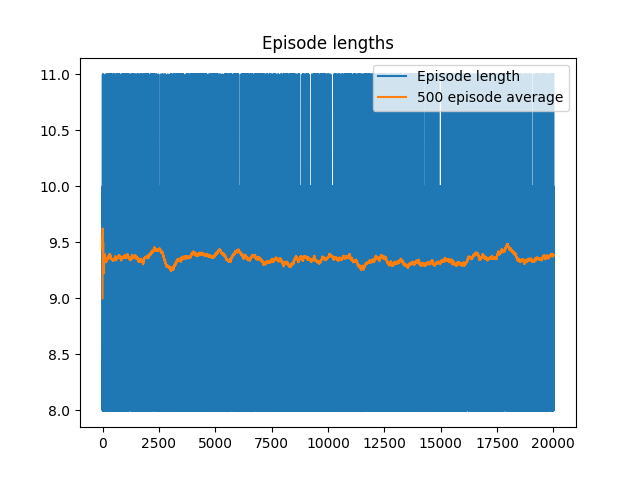
\includegraphics[width=0.9\linewidth]{exercise-3/plots/episodes-fixed-0.0-q0-50.png}
     \caption{Heatmap of the optimal Q-value for variable $\epsilon$}
     \label{fig:task-2-2}
   \end{minipage}
\end{figure}

\subsection{Question 2: Based on the results you observed in Task 3, answer the following questions:}

\subsubsection{In which case does the model perform better?}

In both cases, the algorithm performed extremely badly. It does not achieve any improvement in all the execution period, generating an almost plane line of average timesteps for all the training. \\

If we observe the results of the execution, we can also see that the model did not learn the desired behavior. On the contrary, it gets stuck in the middle of the screen without balancing the pole.

\subsubsection{Why is this the case, and how does the initialization of Q values
affect exploration?}

This situation happens because the agent in most of the cases chooses the same actions, which are maximized, but never explore other possibilities which can lead it to promising results. This can also be seen in the heatmap plot of the optimal q-values (Figure \ref{fig:q2-2}):

\begin{figure}[h]
    \centering
    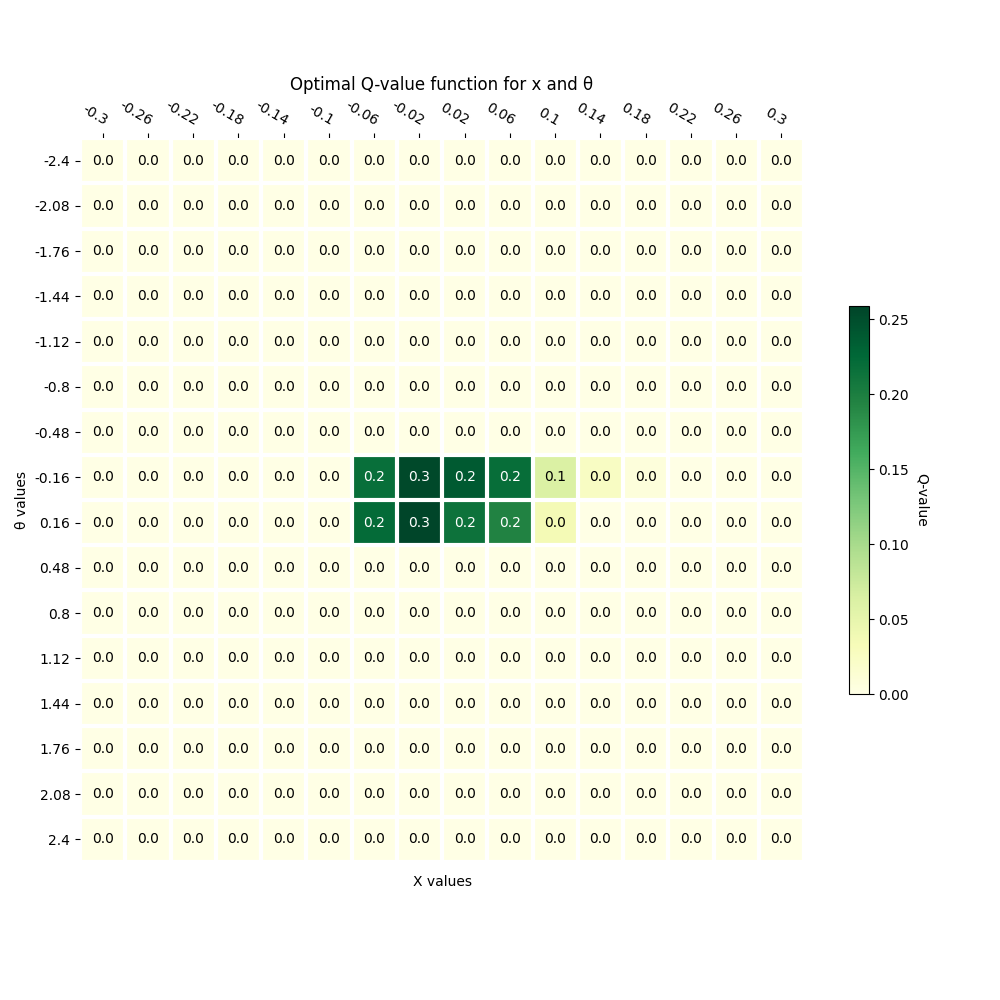
\includegraphics[scale=0.25]{exercise-3/plots/heatmap-fixed-0.0.png}
    \caption{Heatmap for $\epsilon=0$ and $q_0 = 0$}
    \label{fig:q2-2}
\end{figure}

In this plot, only night states in the middle of the board have a value different than zero, and they are not enough for the agent to learn how to balance correctly the pole. \\

The initialization of the grid with the value 50 is not useful in this case, because it is only a re-scale of the initial values, but for the purpose of the agent, all the states at the beginning are equally good. This leads to the same process as if they were initialized to 0.

\section{Lunar lander}

\subsection{Task 4: Modify your code for Task 1 and try to apply it in the Lunar lander environment.}

After modifying the first exercise for the execution of the Lunar Landing environment, we have executed the training of the agent using fixed $\epsilon=0.2$ and using GLIE, obtaining these plots as a result:

\begin{figure}[ht]
    \centering
   \begin{minipage}{0.48\textwidth}
     \centering
     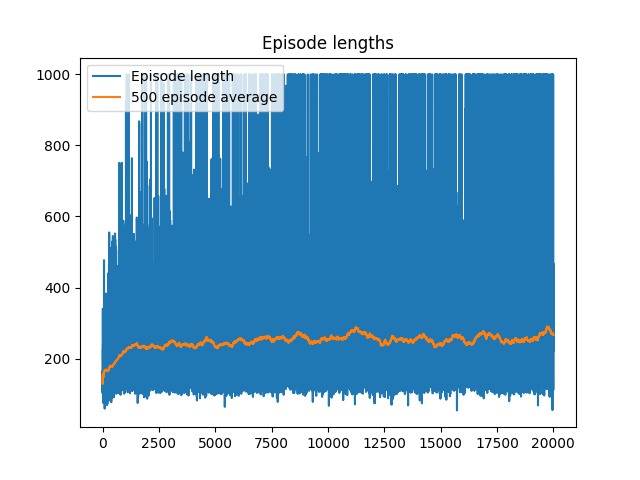
\includegraphics[width=0.9\linewidth]{exercise-3/plots/lunarlander-episodes-fixed-0.2.png}
     \caption{Plot of the average timesteps in training for $\epsilon=0.2$}
     \label{fig:task-2-1}
   \end{minipage}\hfill
   \begin{minipage}{0.48\textwidth}
     \centering
     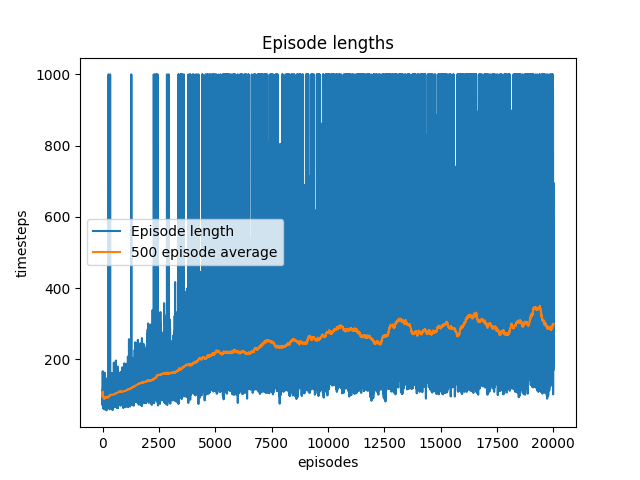
\includegraphics[width=0.9\linewidth]{exercise-3/plots/lunarlander-episodes-variable-0.0.png}
     \caption{Plot of the average timesteps in training for GLIE}
     \label{fig:task-2-2}
   \end{minipage}
\end{figure}

\subsection{Question 3.1: Is the lander able to learn any useful behaviour? Why/why not?}

After the execution, of the lunar lander environment with fixed $\epsilon$ and with GLIE, it can be concluded that the agent is not able to learn the desired environment. \\

In the execution we can see that the agent approximately learns how to remain stable in the air, but can not land appropriately. The technique that we have used for training the lander is based on dynamic programming (saving states in a table), so it has not enough information for learning complex patterns. In addition to that, we have to point out the complexity of the problem, which depends on eight different variables, on the contrary to the cart pole, which only depends on four.\\

This is why usually other techniques based on deep neural networks are used (For example, Deep Q-Learning \cite{deep-q-learning}) because they are able to generalize more complex patterns.

\bibliographystyle{ieeetr}
\bibliography{bibliography}  % Modify template with your bibliography name
\end{document}
